\chapter{中国未来怎么走?}


笔者认为马克思足够深刻地揭示了现代世界的破坏性,但在建设性上乏善可陈,宏观或
曰大师叙事40余年来也欠缺实质性发展,高中学历的笔者也更加无力去探讨中国未来发
展路径应是怎样,但自认可发现个别“忧国忧民”“专家”政策提案所描述美妙画卷背
后隐藏的真实破坏性——一些可以让党和国家陷入大崩溃泥沼、让人民生活日益困苦的
破坏性。笔者确信这个别“专家”要么是天真幼稚的蠢,要么是为背后利益集团服务的
刻意为恶。

当代世界的批判武器虽然在宏观和建设性上缺失,但历经200多年积累,其数量却不少,
可称是批判武器军火库了。边沁利己资本主义的侵蚀,人民批判意识日益增长,信息化
传播越来越便捷,使我们的一些“专家”话术相当高明,可以十句话九句真,隐蔽性极
强。他们九句真话,主要立足批判现实存在的问题、弊端,也常常以人民的名义批判政
府,悲天悯人真是我见犹怜,比如减少城乡二元对立——户籍改革;加大民生支出、社
会保障。但剩下的那一句假话,才是其话术“\textbf{精华}”所在,前面的真话只是语言上
的“合理性”本身,并不会在其政策指导下实现,悄悄引导党和国家、人民成为其背
后利益集团待宰的羔羊。

沽名钓誉、伪道学家、祸国殃民、宵小鼠辈式的“专家”真不少,道行更高者甚至可以
十句话十句真,比如可以流涕于中国财富分化之严重,摇旗呐喊中国要建立健全对富人
的累进直接税征收,呼吁国家招纳这类方向的专家进入智囊团,他自己其实却在国际金
融寡头公司从事着“资本外逃”或者资本管理类的业务……真是让人叹为观止!高手
啊!“高级知识分子”啊!

笔者曾经真的失望于中国脊梁式的专家为何如此罕见,后来在写作本书、搜集资料的过
程中发现自己可能想错了。中国脊梁一样的专家不是凤毛麟角,只是他们大多乏名少利,
影响力有限……不过当前世界已经面临习总书记所说“百年未有之大变局”,脊梁们还
是能发声的多发一些,能做事的多做一些,晚一些隐退于浊世吧……

本节一是说明世界各主要经济体在“百年未有大变局”中的共性背景,二是以《大国大
城》为例,对其批判,希望读者能够多些批判性思维,勇敢独立思考,谨防新自由主义
对公民权利的损害。三是建议党和政府对政策提案要进行不可行性研究,并提供部分考
量标准。四是对中国影子政府业已形成的担忧。


\section{背景:资本主义民主国家危机的共性}


沃夫冈·斯特里克《资本主义将如何终结》\cite{JJDK201504024}\cite{streeck2017will}摘
抄:\improve[inline]{此书引用内容可进一步提炼总结,也可参考豆瓣宫野志保对本书
  的评论。 }
\begin{quotation}
  20 世纪 70 年代的\textbf{全球通胀}之后,发生了 80 年代\textbf{公共债务的上升},而 90 年
  代财政的巩固伴随着这一时期\textbf{私人债务的迅速增加},危机最终在2008年的金融危机
  中爆发,这种紧张局势被一个\textbf{不可持续的“向未来借款”}的过程所取代……40 年
  来,\textbf{失衡}几乎是各“发达”工业国和“发达”工业世界的常态。实际上,随着时间
  的流逝,人们已经不再把危机看成是纯粹的经济危机。这引发人们重新发现资本主义
  社会从前的概念——\textbf{资本主义是一种从根本上依靠私有资本积累连续过程的社会秩
    序和生活方式。}

  了这一趋势;\textbf{二是主要资本主义国家整体负债程度普遍而持续的上升},40 年来,
  这些国家的政府、家庭、金融以及非金融企业不断累积起大量债务;\textbf{三是几十年来,
    伴随着债务增加和经济增长下降,收入与财富分配的不平等均处在上升过程中。}

  多年来,这三者似乎已经相辅相成:低增长加剧了分配冲突,加剧了不平等;不平等通
  过限制有效需求来抑制增长;高额的现有债务堵塞了信贷市场,增加了金融危机的可能
  性;过度增长的金融部门既是经济不平等的结果,也是经济不平等的加剧,等等。

  现在很清楚,资本主义世界的民主国家不是一个主权国家,而是\textbf{两个主权国家:下
    层的人民和上层的国际“市场”。}全球化、金融化和欧洲一体化削弱了前者,加强
  了后者。现在,权力的平衡正迅速向高层转移。\textbf{以前,领导人需要了解和使用人民
    语言;今天,他们必须掌握国际“市场”这一金钱语言。“人民耳语者”由“资本
    耳语者”接替。资本期望领导人知晓可保障投资者以复利收回资金的秘密戏法。}

  \textbf{资本主义可以由于过于成功而破坏其自身。}我所想像的资本主义终结,是资本主义
  由于其自身的原因而慢性衰败的过程。虽然我们\textbf{无从准确知道}资本主义什么时候消
  失、如何消失、以及替代资本主义的将是什么制度,\textbf{但重要的是,目前没有力量能
    够扭转经济增长、社会平等和金融稳定的恶化趋势并终结三者之间的相互强化}。

  当今经济和社会混乱背后存在着\textbf{结构性紧张和矛盾,社会科学几乎无能为力帮助解
    决这一问题。然而,它所能做的是揭示它们,并指出其历史连续性,以便充分理解
    当前危机。}它可以,并且必须指出\textbf{民主国家正在戏剧性沦为全球投资者寡头集团
    的债务催收机构}……今天,经济权力似乎比以往任何时候都更加成为政治权
  力\footnote{笔者注:新自由主义所要求的是经济自由优于政治自由。笔者妄论,可以认为新
    自由主义要求经济权力大于政治权力,政治权力沦为经济权力附庸。},而公民似乎
  已被完全剥夺了自身捍卫民主的力量,以及向政治经济施加影响的能力;公民的利益
  及其诉求与资本所有者的无法相提并论。事实上,回顾1970年代以来的一系列资本主
  义危机,仿佛真的有可能在发达资本主义中找到一种新的(即使是暂时的)社会冲突解
  决方案,这一次完全有利于现在牢固地扎根于其政治上无懈可击的据点——\textbf{国际金
    融资产阶级}。\todo[inline]{笔者对“事实上……”这句话的理解和翻译有问题,
    希望读者能提供中译版原文或者更好翻译。}

  % 公共支出的债务融资必须被对自由化赢家的收入和资产进行更有效的征税所取代。国
  % 家不应再用借来的钱来执行其公民为整个社会规定的任务,然后必须连本带利地偿还
  % 贷款人,而贷款人又将其剩余的财富留给子女。只有扭转社会分裂加深的趋势——资
  % 本主义在20世纪末和21世纪初的标志——才有可能使现代社会摆脱通过无节制地生产
  % 有毒资产来设计合成增长来确保国内和平的强迫。
\end{quotation}

\section{大国大城=超级资本原始积累}

\subsection{大国大城概述}

陆铭写了《大国大城》,概括来说,他希望“在集聚中走向平衡”,政府发力发展节约
空间和时间的\textbf{大城市规模集约经济}——户籍改革,劳动力自由流动;大城市不怕大不
怕扩建,敞开发展并吸纳劳动力,实现人员高度集聚的规模经济。

“拥挤Time、污染Grime和犯罪Crime问题这三种“城市病”对于中国来说并不可怕,事
实上可能并不严重。大城市在合适政府政策下也不会陷入贫
民窟拉美化,且更应去实现高密度基建。

过往土地金融导致地方以邻为壑、各自为政,重复建设、高大全项目体系可以休矣。当
然,这点批判完全没有问题的,许多专家也痛陈这一弊端,本书也涉及,这已是一种定
论。

\subsection{具体批判}

笔者无意于多么科学详实、引经据典地说明自己的批判观点,对于这样错漏百出、昭然
若揭的书来说并无必要。

接下来笔者逐条引用《大国大城》陆铭观点,然后进行具体批判:

\begin{enumerate}

\item 无知之幕
  \begin{quotation}
    美国的政治学家罗尔斯在他的《正义论》当中提出,一个问题中所涉及的所有各方,
    都应该被放在同一个标杆之后,在那儿\textbf{没有角色之分,也没有社会差异},这样的
    原则被称为“\textbf{无知之幕}”(veil of ignorance)。更通俗地说,其实这就是国
    际版的“换位思考”和“己所不欲,勿施于人”,这意味着在公共政策的讨论当
    中,\textbf{每一个公民所持的观点应该与自己的社会身份无关。}再换句话说,\textbf{公民所
      持的观点不应该跟自己是否在当前处于既得利益的位置有关。}


    中国的地方政府最大化本地利益,缺乏彼此之间的协调,国家利益被忽视,这极大
    地影响了中国发展的道路和可持续性。\textbf{中国已经到了呼吁每一个省、每一个市、
      每一个县、每一个人放弃本地思维,顾全公共利益的时候了。}(中央的更加集权,
    行政性配置,是否可能?地方不均衡如何解决?落后地区如何照顾?)


    不管是通过\textbf{财政转移支付}的方式,还是通过\textbf{帮欠发达地区还债}的方式,\textbf{发
      达地区都需要负起相应的责任}。读者可能会问,发达地区为什么要负起这个责任?
    道理并不复杂,因为这是\textbf{统一国家的必需},而且,发达地区恰恰是因为处于一个
    统一国家和统一货币区的内部,享受了统一市场的好处,获得了来自欠发达地区不
    断流入的劳动力资源,并且恰恰因为自身是这个国家统一货币区的一部分而成了金
    融中心。\textbf{只想要统一的好处,不想承担统一的义务,这是任何国家的政治都不会
      允许的。}
  \end{quotation}

  “无知之幕”本身没有错,但当前世界不正是笼罩在功利利己这一经济学倡导的“理
  性”之下么?从何让各级组织和个人放弃自利,去实现这无知之幕呢?中国如何呼吁
  和管控? 级级以邻为壑,事权层层下压,财权层层上收的过去,一下子变成大同天下,
  统一大国。真好!共产主义一夜间到来了么?真是正确又毫无营养的梦话。

  陆教授知道“\textbf{发达国家才不会以天下大同为己任呢!}”但似乎不知道自由经济学家们
  口中所说的利己“理性人”,不止包括人,也实际包括着各处各级人的组织。

  我们回到恩格斯《论住宅问题》,看到了历史的轮回:

  \begin{quotation}
    现代的国家不能够也不愿意消除住房灾难。国家无非是有产阶级即土地所有者和资
    本家用来反对被剥削阶级即农民和工人的有组织的总权力。\textbf{个别资本家}\footnote{恩格
      斯注:这里与问题有关的只是资本家,因为\textbf{参加这种事业的土地所有者首先也
        是以资本家资格出现的}}\textbf{不愿意做的事情,他们的国家也不愿意做。}因此,
    如果说个别资本家对住房短缺虽然也感到遗憾,却未必会受触动而去从表面上掩饰
    由此产生的极其可怕的后果,那么,总资本家,即国家,也并不会做出更多的事情。
    国家顶多也只是会设法在各地均衡地推行已经成为通例的表面掩饰工作。我们看到
    的情形正是如此。
  \end{quotation}

  笔者知道,资本和性质等问题较为敏感。这里主要请读者理解。诚然,资本主义不完
  美,相当具有破坏性,但至今仍是革命性的和先进的,尚未有可以取代的生产关系。
  过去的所谓社会主义其主体是国家垄断资本主义,社会主义或许只是一个空想,并不
  具备多少科学成分。中国不能不走向这条道路,不然早就崩溃,只是我们走的太快太
  快。本章首节引用了沃夫冈·斯特里克的几段话。在他看来,马克思可能悲观
  了,\textbf{资本主义如今日益严重的危机可能在尚未有新的革命性生产关系出来之前终结}。
  笔者对此抱有怀疑,斯特里克可能乐观了。

  至于国家,也请理解这番直言。笔者只是一介草民,于国于家无用,身无长物;没有
  加入什么结社团体;更无什么图谋不轨。只是世界各国如今都太危险了,中国作为各
  大国强国眼中的大肥肉,皆欲分我血肉、食肉寝皮,更是危险中的危险;而国外垄断
  金融寡头对我国的侵蚀程度并不乐观,国家自然肯定有相关了解。当前资本主义危机
  如此严重,正有没有了竞争意识形态的压力这一原因。我要说出来,便想给出一个小
  压力,使国家不至于那么乐观,政策后果不至于那么坏,能减轻一些就好。

  \todo[inline]{以上部分太尖锐?删减?}

\item 用人均GDP、人均收入和生活质量来考量区域平衡

  \begin{quotation}
    应该从GDP总量增长的考核转变为人均GDP的考核。特别是对那些人口流出地来说,
    追求人均GDP、人均收入和生活质量才是长久之计,

    经济学家的研究发现,在欧洲,收入不平等减少快乐,而在美国,这种效应却不强。
    这实际上就和美国社会不同收入阶层之间的流动性更强有关,其实,\textbf{“美国梦”的
    道理就是说每个人都平等地拥有致富的机会}。
  \end{quotation}

  前文已述(见\cref{sec:gdp}),GDP、总收入的加总方式,无法说明分配不均、贫富
  差距、社会福利这类问题。大区域(比如美国的州)人均的本质仍是加总,同样无法
  说明这类问题。陆铭进而通过美国各州人均GDP比较平衡,证明美国区域发展均衡。美
  国梦“每个人都平等地拥有致富的机会”,哈哈哈哈……美国财富不平等可
  见\cref{tab:gini}。

\begin{figure}[ht]
  \centering
  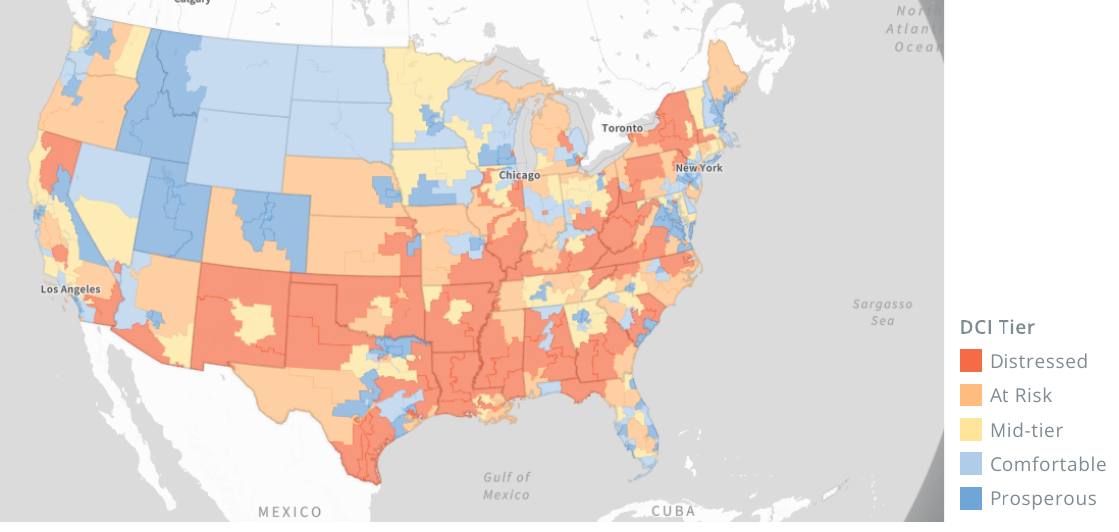
\includegraphics[options]{figures/DCIbyDistricts.png}
  \caption{\label{fig:DCIbyD}美国困境社区指数(按districts划分)}
  \capsource{来源:\href{https://eig.org/distressed-communities/}{美国经济创
      新集团}}
\end{figure}

也可以参考美国经济创新集团(The Economic Innovation Group)发布的困境社区指数
(DCI,the Distressed Communities Index,见\cref{fig:DCIbyD})\footnote{对困境社区指
  数DCI的中文介绍可见澎湃 《美国社区评价:困境社区指数和繁荣城区体系》。}。
\change[inline]{可以根据以上DCI链接网址,进一步阐述美国区域不平衡。}

  \begin{quotation}
  但是,城市化和地区之间的自由移民是一个\textbf{几十年甚至上百年的过程},在这个过程
  中,如果我们只看\textbf{特定时段的局部地区},就可能会觉得,劳动力流动并没有带来地区
  间收入水平差距的缩小。
  \end{quotation}
  陆铭倒是知道这是即使均衡,也需长期。可在几十年甚至上百年的区域失衡中,中国
  中央和地方、地方和地方、政府和人民的矛盾恐怕早已内爆了。

\item 不可能三角

  \begin{quotation}

    第一,国家的统一。

    第二,经济效率的提高。

    第三,区域之间的平衡发展。

    大国发展的“\textbf{不可能三角}”,而如果要破解这个“不可能三角”,就必须改
    变“平衡”的定义,将经济资源和人口均匀分布意义上的“平衡”,转变
    为\textbf{人均GDP、人均实际收入和生活质量意义上的“平衡”},而这种人均意义上的
    平衡恰恰是可以在人口自由流动的过程中实现的,不需要大规模地采取行政控制的
    手段来对人口流动进行限制。
  \end{quotation}

  前面一条已述人均“平衡”的荒谬。那么按陆铭说法,我们还是要面对不可能三角。
  我们是要国家的统一,还是经济效率的提高,还是区域之间的平衡发展呢?事实上会
  走到哪一步?

  恐怕这三角三边全部失败,只留资本寡头的胜利,他们可以资本外逃或当买办。

\item 地方比较优势

  笔者呼吁国家和人民一定要小心对待任何“比较优势”的说法!比较优势基于区
  域\textbf{特殊}性,神马生态农村、农家乐、旅游、港口,能覆盖和折射中国多少区域?


\item 政府支出和中央转移支付

  我们的陆教授说了几句冠冕堂皇的话,既好听又正确!那在现实情况下,其真正的意
  图或会导致的结果是什么呢?

  % \begin{quotation}
  %   \textbf{社会保障健全}则储蓄的动机将减弱。
  % \end{quotation}

  % 正确。我们的社会保障体系健全吗?有多少人交养老、医疗保险?增长率如何?政府
  % 要投入多少?另外,储蓄是世界银行、世界货币基金组织和一些国内外经济学家等长
  % 期、屡次建议我国采取政策使居民降低储蓄,我国也有提出可用“六个钱包”付房子
  % 首付的官员。储蓄对于我国大部分居民来说是风险经验所得。减少储蓄的目的是刺激
  % 投资,“经济发展”……

  \begin{quotation}
    农民在放弃土地的时候要满足\textbf{自愿、有就业、有社会保障、土地(或建设用地指
      标)能够市场定价这几个基本的前提},让农民避免被剥夺。而以禁止市场交易的
    方式来保障农民,这是最为荒谬的逻辑,其结果恰恰是给不尊重土地产权的行政性
    剥夺找到了借口。(农业税?羊吃人?农业工业化的挤出)
  \end{quotation}

  真好听!“自愿、有就业、有社会保障、土地(或建设用地指标)能够市场定价”四
  个前提能达成肯定没问题,好事一桩!

  只是四个前提很可能一个都实现不了。

  普遍劳动力过剩的情况下,让农民挤入城市谋生,小城市市民挤入大城市,集约规模
  经济下,劳动力只会更加溢出,产业后备军必然更大,失业劳动力更多!如何保障就
  业,人口流出小城市难以维持,农民又如何自愿前往城市?如何保障农民、职工的社
  会保障?肯定要政府支出,我们现实的社会保障是什么水平,要达到这个目标又需要
  什么水平呢?不知从何而来的巨额支出!

  土地的市场定价,呵呵,恐怕是软硬暴力下才会有这一市场吧。这条放在本节总结时
  再论述总结。


  通过\textbf{中央向地方的财政转移支付,可以为人口流出地的养老提供更多资源。}更重要
  的是,\textbf{全国的养老保障体系将逐步走向一体化},这时,即使人口流出地面临更为严
  重的老龄化问题,也不需要担心了,这才是解决问题的根本出路。

  中国城市的土地是国有的,这在根本上可以允许\textbf{中国城市政府作出更好的规划},以
  及\textbf{向低收入居住区提供基本而必要的公共服务,来防止大面积贫民窟的出现。}

    在“蛋糕做大”的情况下,中央财政就更有能力来进行\textbf{区域间和城乡间的财政转
      移},但未来的财政转移应该更多地用于\textbf{城乡和区域间公共服务的均等化},比
    如说提高欠发达地区中小学教师和医护人员的待遇,相应地减少欠发达地区(特别
    是农村)政府的财政负担,以促进区域和城乡间在生活质量上的平衡,实现“动
    人”和“动钱”的良性互动。


    如果一个城市可以通过基础设施和人力资本的投入,从而放大正外部性,会引导城
    市进一步向有效的更大规模城市发展;如果一个城市可以通过技术进步和政府的管
    理措施减少负外部性,也可以使这个城市更加有效地运转。
  \end{quotation}


  结合现实状况(\footnote{不能结合现实的政策提案,有什么用呢?},其所要求的是什么?
  中央承担全民社会保障,以“自愿、有就业、有社会保障、土地(或建设用地指标

  (“资本家不愿做的事,政府也不愿做”,为什么不让资本家去做呢?因为外部性?
  可实际上在历史经验及现实情况下,前者是政府的持续赤字,后者是太过乐观——政
  府的无能为力(包括美国))

  地价和房价本身就成为低效率企业和劳动力进入大城市的障碍,这就是市场的力量。

\item 持续发展


城市部门是不是能够持续地提高生产率,并为农村进城的移民源源不断地创造就业,


避免城市出现贫民窟问题的关键是要通过城市发展源源不断地为进城农民创造就业机会,

\item 发展消费型服务业

  给定一个国家劳动力的教育水平,反而使大城市吸引大量的低技能劳动力前去工作。


  服务业岗位,从而吸纳更多的农村人口进城,使得城市化率不断提高,直至75%,甚至80%以上的水平。

  餐饮、家政、网约车、快递、外卖


  并且为其提供适度的公共服务和社会保障。\improve[inline]{future应包含贫民窟的考
    量}

  对于部分国家出现的贫民窟现象,要作有针对性的分析。城市经济是否可以持续增长,
  从而为农村移民创造就业是非常重要的问题,一些拉美国家经济增长乏力,制约了低
  收入阶层提高收入的机会。而在印度这样经济增长较快的国家,城市经济高度偏向现
  代服务业和信息技术产业,为低技能者创造的就业机会有限。


\item 农业工业化

  集聚意味着生产力的高度发达,需要的人工越来越少
  要让其致富,关键的措施就是减少人口,给钱还是次要的。

  随着农民不断减少,剩下的农民从农民变成规模化经营的农场主,或者农场里的“农
  业工人”,收入也将提高。制约农业发展的瓶颈要素是土地,土地是不可能无限增加
  的,所以一旦土地决定了农产品的增长极限的时候,要提高农民的人均收入只有减少
  农业人口,这在卓玛与松茸的故事里也讲过。而工业和服务业的发展却可以不断地进
  行资本积累,不断地创造就业。

\end{enumerate}

% 集聚也的确会带来坏处,比如说拥挤、污染和犯罪。当集聚带来的好处不够高,而坏处体现出来之后,集聚的水平就相应地稳定下来。而在这个过程中,非常重要的调节变量就是生产要素的价格,集中体现在地价、房价和劳动力工资上。


内部的全球化流动 或者 中国地区化


% 一方面,对于市场上的债务违约,中央当然希望打破“刚性兑付”的预期,以免将什么责任都揽在中央,让人们形成地方债务没有风险的预期;另一方面,面对事实上已经难以偿付的地方债务,最终还是会被认为将由中央政府来兜底,从长期来看,这也恰恰可能造成地方政府不计后果地借债的局面,这就是经济学里典型的“道德风险”问题


% 世界主要经济体基尼系数基本已达70以上,无论是国家人均还是大地区级的人均GDP这两
% 个指标已难以说明其中人民的经济水平,它们更能说明的只是富人资本。

% https://m.thepaper.cn/newsDetail_forward_22666274

% 吸纳不了,黄奇帆 美国 金融华尔街30万人



% 发达国家才不会以天下大同为己任呢!所以,发达国家的政策一定是只要高技能人才,低技能劳动力他不要。

% 高收入、好的公共服务,伴随着相对严重的“城市病”和高房价,其实恰恰是地区间生
% 活质量平衡的表现。不过,我还要强调一下,这里说的“城市病”在一个国家内部成为
% 生活质量平衡的机制,是指横向的比较。在本书的下篇中,我们还会说到,从历史的维
% 度来看,城市人口规模的扩张并不一定伴随更为严重的“城市病”,“城市病”可以通
% 过\textbf{技术和管理的手段}来解决。


% 沿海到中西部买这个土地指标…… 随着建设用地指标的跨地区再配置(可看下央地关系重庆模式的问题再行批判)


% % 分别有67.2\%和63.2\%的新生代农民工认为“{\bf 收入太低}”和“{\bf 住房问题}”
% %           是制约在城市定居的重要困难和障碍。所以,{\bf 政府可以做的是为有定
% %           居意愿的农民工创造条件,而不是以农民没有进城意愿作为借口放缓城市化}。






% 我并不是反对为欠发达地区提供财政补贴,我要讨论的是,在政府进行财政转移的时候,
% 应当考虑转移的数量、地点和结构,如果违反市场经济的规律,盲目追求人口和经济资
% 源的均匀分布,那么,一系列低效率的后果就必然会出现。

% 西部和边陲的发展,因为这是政治和国防的问题,但政治和国防与我们这里讨论的问题没什么关系。

% 2014--2020新型城镇化规划只是北京、上海超大城市限制发展。

% 若人口不从欠发达的地区流出,就很难提高这些地方的劳动生产率。中国总有一天会达
% 到75\%以上的城市化率。如果制造业和服务业能够不断地加强国际竞争力,不断地创造
% 就业,那么中国的城市化率达到80\%以上也并非不可能。在这个过程当中,随着农村人
% 口的减少,农业的劳动生产率必然不断提高。不用过于担心农村人口的减少会危害农业,
% 恰恰相反,人口的流出是农村地区提高规模经营程度和劳动生产率的前提条件。随着空
% 心村现象不断发展,一部分的农村社区将逐渐消失,原有的宅基地不断空出,复耕为农
% 业用地,现有的一家一户的农业经营模式就将逐渐转变为大农场的模式,这样,农民的
% 收入水平才可能不断提高。只有规模经营才能让农业成为能够致富的产业,才可能让一
% 部分人愿意留在农村当农民。不同的是,未来的农民和现在的农民含义就不一样了,他
% 们应该受教育水平更高、更年轻,才能适应经营大规模农业的需要。

% 在转型期,由于公共服务的享受权仍然与户籍身份挂钩,同时,在公共服务供给不可能短期内快速增长的情况下,改革不能在一夜之间取消户籍与公共服务的挂钩,因此,户籍的转换或者特大城市实施的积分落户制度就必须设置门槛,形成对于一部分人的事实上的公共服务歧视。那么,这样过渡时期的“歧视”应该遵循什么原则?这就要本着理性原则,尽量将仅仅为公共服务而流动的人口识别出来。

% 因此,政府可以通过一定的办法来识别出仅仅为了公共服务而迁移的人群。其中,最好的办法就是认为有就业记录和社会保障记录的人群是以就业为主要目的的迁移人群。虽然这一标准并不完美,却是现行条件下能找到的最好指标。










% 1、美国的“地多人少”是通过屠戮原住民获得的大片土地,每一块土地下面都有印第安人的尸骨。而我们本身就是原住民,脚下的土地是由我们共同的祖先开拓的土地,再大的利益也不能将屠刀挥向同胞。

% 2、美国的“农民”也不是我们常识中的农民,而是农场主,或者说“地主”

% 本节以陆铭《大国大城》
% 为例展开批判,并非因为陆铭是段位很高的“高级知识分子”或很专的“专家”。相比
% 于他那些可以十句话里九句真、只有一谎为利益目的的同路“专家”,他的话术并不高
% 明,往往以片面论述全面,以个别论证一般,以小作文抒情代替论证,但其“大国大
% 城”政策提案却真是太可怕了,这是赤裸裸的“超级资本原始积累”……


% 尊重的规律是什么?是有权势者对无权势的尽情盘剥。

% 社会保障健全则储蓄的动机将减弱。

% 经济学家的研究发现,在欧洲,收入不平等减少快乐,而在美国,这种效应却不强。这实际上就和美国社会不同收入阶层之间的流动性更强有关,其实,“美国梦”的道理就是说每个人都平等地拥有致富的机会。

% 中国城市的土地是国有的,这在根本上可以允许中国城市政府作出更好的规划,以及向低收入居住区提供基本而必要的公共服务,来防止大面积贫民窟的出现。

% 避免城市出现贫民窟问题的关键是要通过城市发展源源不断地为进城农民创造就业机会,并且为其提供适度的公共服务和社会保障。

% 对于部分国家出现的贫民窟现象,要作有针对性的分析。城市经济是否可以持续增长,从而为农村移民创造就业是非常重要的问题,一些拉美国家经济增长乏力,制约了低收入阶层提高收入的机会。而在印度这样经济增长较快的国家,城市经济高度偏向现代服务业和信息技术产业,为低技能者创造的就业机会有限。

% 中国的地方政府最大化本地利益,缺乏彼此之间的协调,国家利益被忽视,这极大地影响了中国发展的道路和可持续性。

% 经济发展对于空间集聚的要求越来越高,而地方政府却追求本地经济规模和税收规模的最大化。

% ,释放劳动生产率

% 生产要素的充分流动增进社会和谐,将进一步减少经济和社会资源的无谓消耗。

% 本节以陆铭《大国大城》
% 为例展开批判,并非因为陆铭是段位很高的“高级知识分子”或很专的“专家”。相比
% 他可以十句话里九句真、只有一谎为利益的同路人,他的话术并不高明,往往以片面论
% 述全面,以个别论证一般,以小作文抒情代替论证,但其“大国大城”政策提案却真是
% 太可怕了,这是赤裸裸的“超级资本原始积累”……



%%% Local Variables:
%%% mode: latex
%%% TeX-master: "../main"
%%% End:
